\documentclass{article}

\usepackage{ocencfd}
\usepackage{tikz}

\title{Foundations of Cryptography} % Sets article title
\author{Soham Tripathy CS20B073, Saksham Singh CS20B067, Aditya Vaichalkar CS20B084} % Sets authors name
\authorID{cs20b073} %Link to your profile ID.
\documentID{template} %Should be alphanumeric identifier
\fileInclude{} %Names of file to attach
\date{August 24, 2023} % Sets date for publication as date compiled

% The preamble ends with the command \begin{document}
\begin{document} % All begin commands must be paired with an end command somewhere

	\maketitle % creates title using information in preamble (title, author, date)
    
	%New section is created
	\section{Informal Discussions on Pseudo Random Functions}
	%Plain text is just written directly in this document like this:
        \begin{tikzpicture}
              \node[circle, draw] (D) at (0, 0) {D};
              \node[circle, draw] (O) at (9, 0) {O(.)};
			  \draw (D) -- (O);
            \end{tikzpicture}

	%New section about equations
	\section{Equations}
	Here is an inline equation: \ieq{F=ma}. Below is a block equation which we can label as \eqref{example_eqn}.

	\begin{equation} 
		\label{example_eqn}
		a^2+b^2=c^2
	\end{equation}

	%New section about tables and figures
	\section{Figures and tables}
	\figref{figtest} is an example figure. 

	\begin{figure}[h!]
  		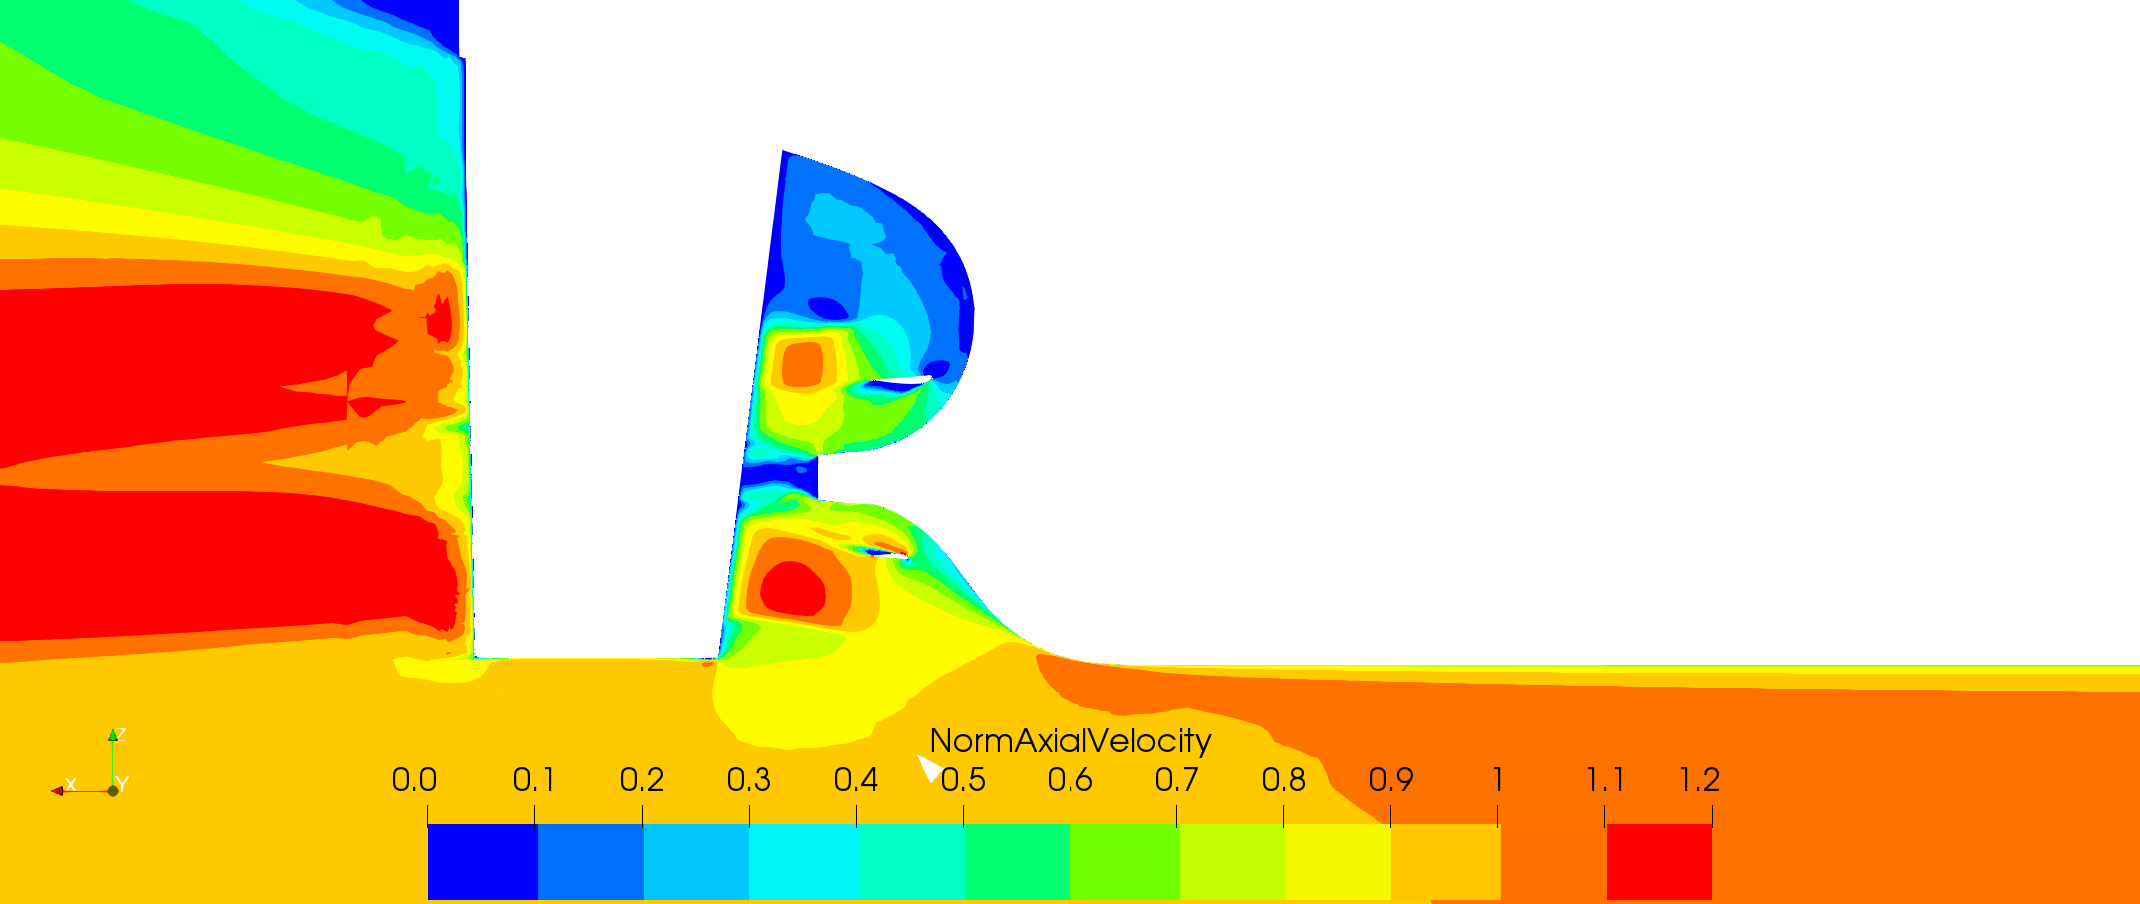
\includegraphics[width=\linewidth]{images/example.png}
  		\caption{An example image.}
  		\label{figtest}
	\end{figure}


	\tableref{tabletest} is an example table.

	\begin{table}[h!]
		\caption{An example table.}
		\label{tabletest}
		\begin{center}
  			\begin{tabularx}{\textwidth}{ X X X }
    				\toprule
    				Heading 1 & Heading 2 & Heading 3 \\ 
    				\midrule
    				1 & 2 & 3 \\ 
    				4 & 5 & 6 \\ 
    				7 & 8 & 9 \\
    				\bottomrule
  			\end{tabularx}
		\end{center}
	\end{table}

	%New section about code
	\section{Code}
	Below is some C++ code.
	\begin{lstlisting}[language=C++]
tmp<fvVectorMatrix> tUEqn
(
	fvm::div(phi, U)
	+ MRF.DDt(U)
	+ turbulence->divDevReff(U)
	==
	fvOptions(U)
);
\end{lstlisting}
   
	
	%Add bibliography at the end of document	
	\bibliography{template}
	\label{bibsect}

\end{document} % This is the end of the document